\begin{frame}{Bayesian Optimization}
  Bayesian optimization provides a principled way for searching optimal
  hyperparameters for a single algorithm. Effective for,

  \begin{itemize}
    % https://dhnzl.files.wordpress.com/2016/12/fuzzymad2016_bo_pdf.pdf
    \item Evaluating each sample is expensive.
    \item The objective is a black-box.
    \item The evaluation can be noisy.
  \end{itemize}

  \begin{columns}
    \footnotesize
    \column{0.5\textwidth}
    Gaining attraction for system tuning:

    \begin{itemize}
    \item CherryPick~\cite{alipourfard2017cherrypick}
    \item FLASH~\cite{zhang2016flash}
    \item BOAT~\cite{dalibard2017boat}
    \item Google Cookie~\cite{solnik2017bayesian}
    \end{itemize}
    \column{0.5\textwidth}
    \begin{figure}
      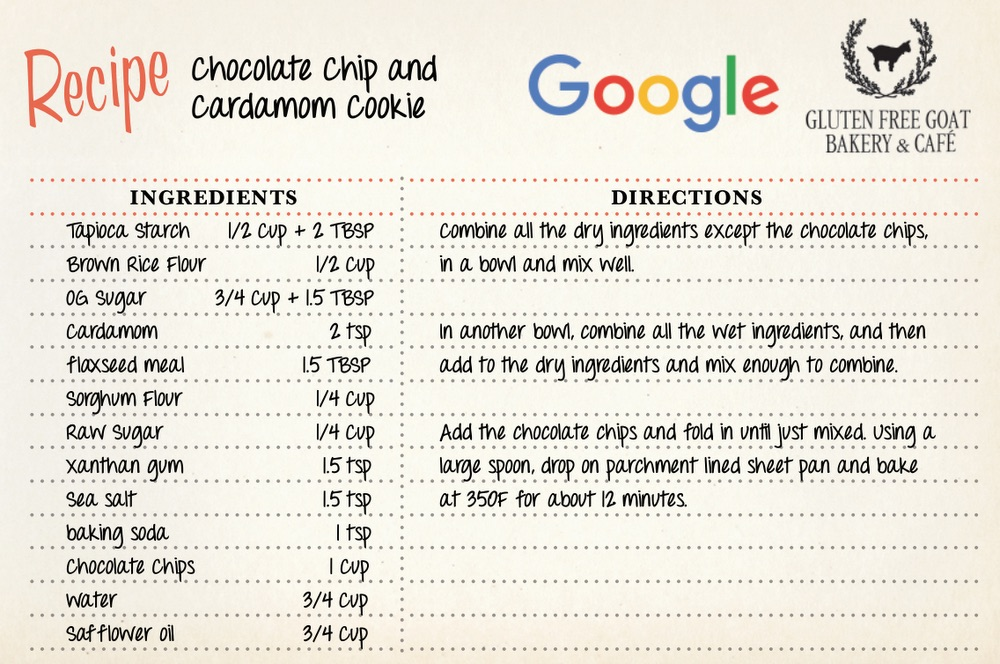
\includegraphics[width=\linewidth]{figures/google-cookie.jpg}
    \end{figure}
  \end{columns}

\end{frame}

\begin{frame}{Bayesian Optimization (Illustrated)}
  \begin{columns}
    \column{0.6\textwidth}
    \begin{figure}
      \centering
      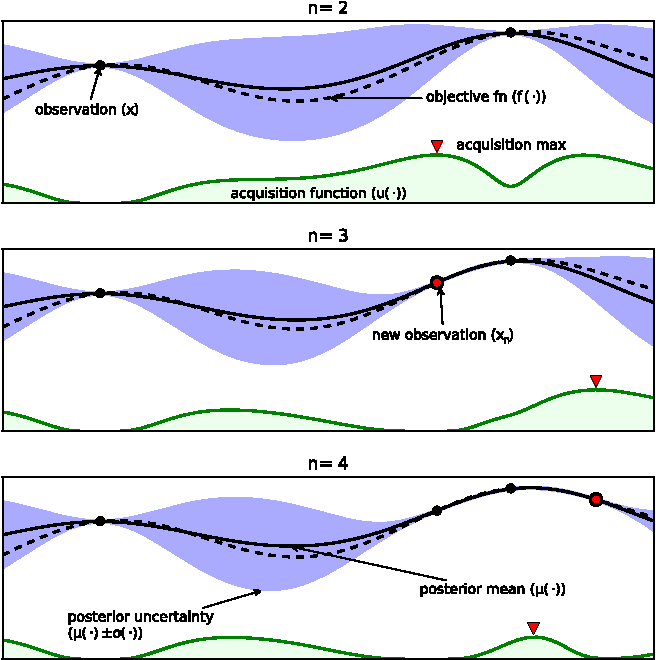
\includegraphics[width=0.8\textwidth]{figures/serving-bo-illustration.pdf}
      \caption{Acquisition function evaluates the utility of candidate points
        for the next evaluation of $f$, balancing a high objective
        (exploitation) and high uncertainty
        (exploration)~\cite{shahriari2016taking}}
    \end{figure}

    \column{0.4\textwidth}
    \begin{figure}
      \centering
      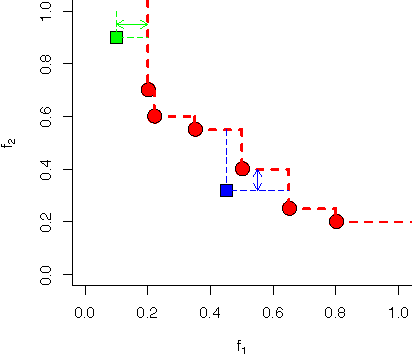
\includegraphics[width=0.8\textwidth]{figures/serving-bo-2d-1.pdf} \\
      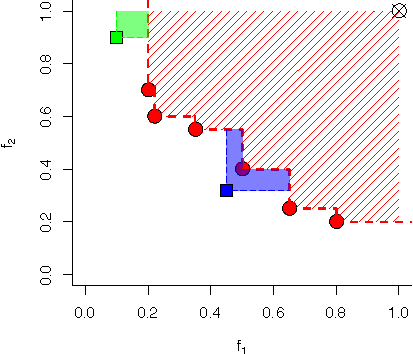
\includegraphics[width=0.8\textwidth]{figures/serving-bo-2d-2.pdf}
      \caption{For two-objective optimization, utility gain is based on
        additive-epsilon (top) or hypervolume (bottom)~\cite{binoisgpareto}}
    \end{figure}
  \end{columns}
\end{frame}

\begin{frame}{Bayesian Optimization For Performance Modeling}
  \vspace{1em} We use PESMO\footnote{It chooses evaluation points to maximally
    reduce the entropy of the posterior distribution over the Pareto
    set.}~\cite{hernandez2016predictive} and compare it with two baselines: (1)
  greedy/coordinate search; (2) random search.

  \pause
  \begin{figure}
    \centering
    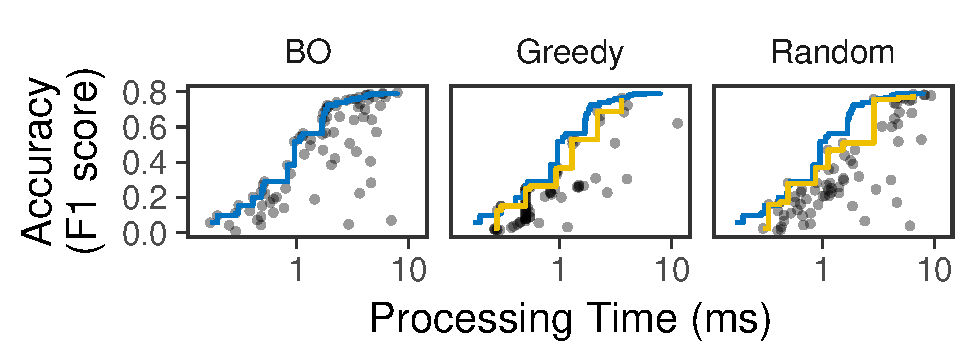
\includegraphics[width=0.95\linewidth]{figures/serving-eval-bo.pdf}
    \caption{BO evaluates 50 configurations and recommends 29 configurations as
      the Pareto-optimal boundary (the blue line). Greedy and Random find
      sub-optimal Pareto configurations with a budget of 80 evaluations (the
      yellow line in each figure).}
  \end{figure}
\end{frame}

\begin{frame}{Cross-Platform Performance Modeling}
  \vspace{1em}
  The profile (performance model) is transferable across machines.
  \begin{itemize}
  \item Accuracy stays the same across machines.
  \item Processing time can be approximated with a linear model.
  \item The ``Pareto-optimal'' is horizontally stretched/compressed.
  \end{itemize}

  \visible<2>{
    \begin{figure}
      \centering
      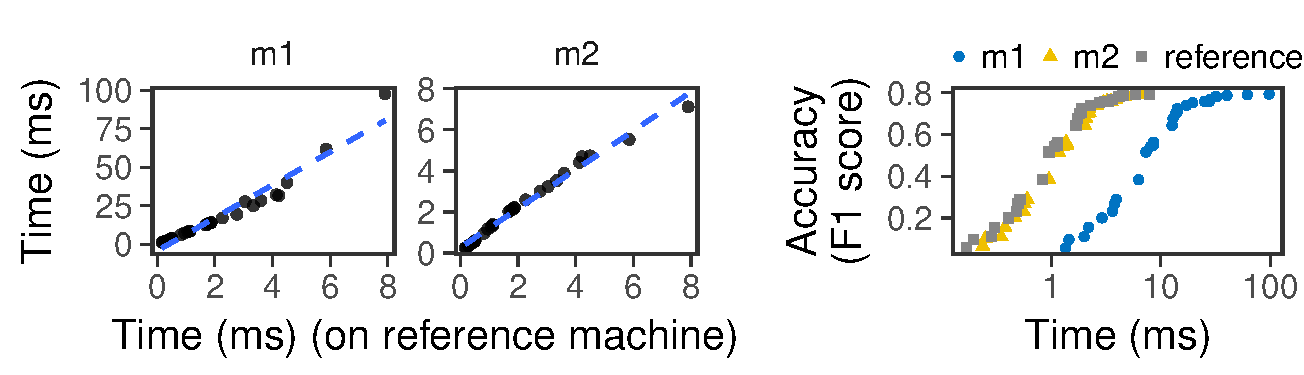
\includegraphics[width=0.95\linewidth]{figures/serving-cross-platform.pdf}
      \caption{(Left) Linear approximation of processing times. (Right)
        Stretched/compressed profile. See paper for details.}
    \end{figure}
  }
\end{frame}

%%% Local Variables:
%%% mode: latex
%%% TeX-master: "../talk"
%%% TeX-engine: xetex
%%% End:
